\documentclass{article}
\usepackage{listings}
\usepackage{xcolor}
\usepackage{caption}
\usepackage{graphicx, subfig}
 \usepackage{float}
\usepackage[utf8]{inputenc}
\lstset{numbers=left, %设置行号位置
        numberstyle=\tiny, %设置行号大小
        keywordstyle=\color{blue}, %设置关键字颜色
        commentstyle=\color[cmyk]{1,0,1,0}, %设置注释颜色
        frame=single, %设置边框格式
        escapeinside=``, %逃逸字符(1左面的键),用于显示中文
        breaklines, %自动折行
        extendedchars=false, %解决代码跨页时,章节标题,页眉等汉字不显示的问题
        xleftmargin=1em,xrightmargin=1em, aboveskip=1em, %设置边距
        tabsize=4, %设置tab空格数
        showspaces=false %不显示空格
       }

\title{Ass2}
\author{Wangzhihui Mei, HongYi Huang, ChangXu, Zijia He}
\date{November 2020}

\begin{document}

\maketitle
\section{Task1}
\subsection{data describe}
Cardiovascular diseases (CVDs) is the leading cause of mortality in India. Ischemic heart disease and stroke are the predominant causes and are responsible for nearly 80\% of CVD deaths. 

\begin{lstlisting}[language=R]
dt <- read.csv("heart1.csv",na.strings = "?")
dt <- na.omit(dt) # handle NA
head(dt)
\end{lstlisting} 

\begin{figure}[H]
  \centering
  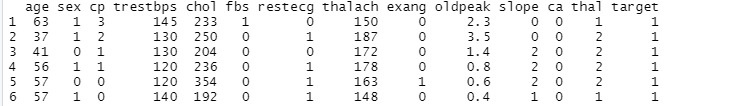
\includegraphics[width=1\textwidth]{task1_1_dtHead.png} %1.png是图片文件的相对路径
\end{figure}
This database contains 14 attributes. The "target" field refers to the presence of CVD in the patient. It is
integer valued 0 (no presence) or 1 (presence). Next we look in detail at the data characteristics of each attribute.
\\
Age: Age in years\\
Sex: (1 = male; 0 = female)\\
CP:Chest pain type(1-typical angina, 2-atypical angina, 3-non-anginal	pain, 4-asymptomatic )\\
trestbps:Resting blood pressure (in mm Hg on admission to the hospital)\\
Chol:Serum cholestoral in mg/dl\\
Fbs:Indicator of whether fasting blood sugar>120 mg/dl (1-true; 0-false)\\
restecg:Resting electrocardiographic results\\
exang:Exercise induced angina (1-yes; 0-no)\\
oldpeak:ST depression induced by exercise relative to rest\\
slope:Slope of the peak exercise ST segment (1-upsloping, 2-flat, 3-downsloping)\\
ca:Number of major vessels (0-3) colored by flourosopy\\
thal:Summary of heart condition(3 = normal, 6 = fixed defect, 7=reversable defect)\\
target:the “The Disease Diagnosis” field refers to the presence of heart disease in the patient(0-No presence,1-Presence) 
\begin{lstlisting}[language=R]
  summary(dt)
\end{lstlisting} 
  
  \begin{figure}[H]
    \centering
    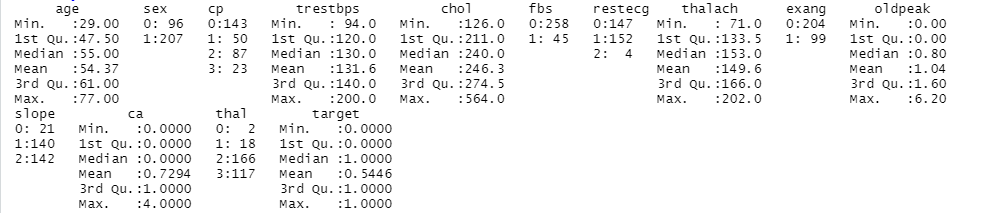
\includegraphics[width=1\textwidth]{task1_1_dtSummary.png}
  \end{figure}

\subsection{logistic regression}
By looking at the details of each data item in the dataset, it was found that the values of age as well as maximum heart rate were quite different and needed to be processed for both data items.
\begin{lstlisting}[language=R]
summary(dt$age)
dt$age<-cut(as.numeric(dt$age),breaks=3,labels=c("low1","normal1","high1"))
levels(dt$age)
table(dt$age)
\end{lstlisting}
\begin{figure}[H]
  \centering
  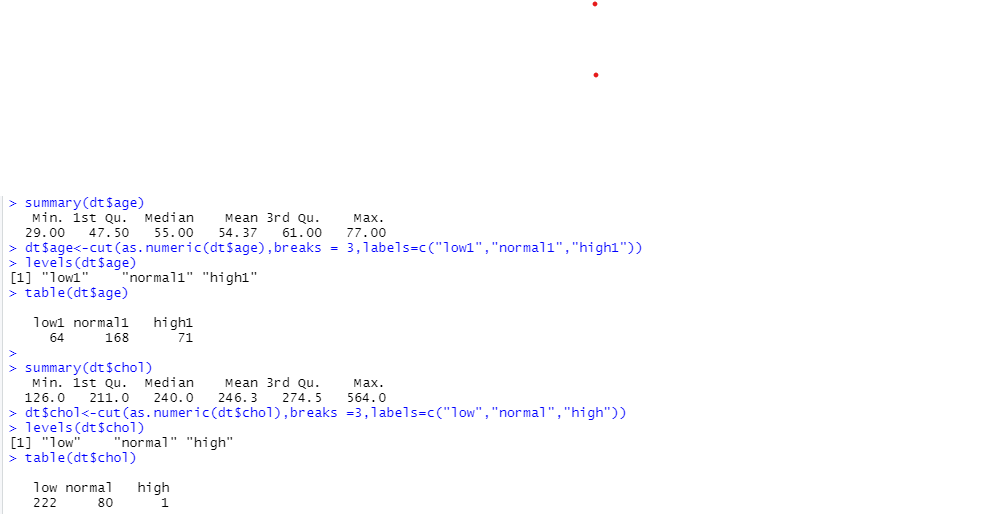
\includegraphics[width=1\textwidth]{task1_1_ageSummary.png}
\end{figure}
Dividing the data set into training and test sets according to a 7 to 3 ratio
\begin{figure}[H]
  \centering
  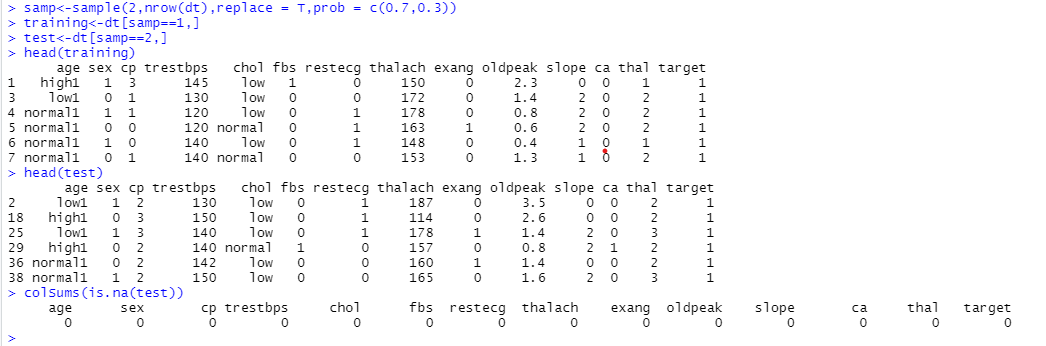
\includegraphics[width=1\textwidth]{task1_1_dataDivide.png}
\end{figure}
Next, a logistic regression prediction model is built using the training set data
\begin{figure}[H]
  \centering
  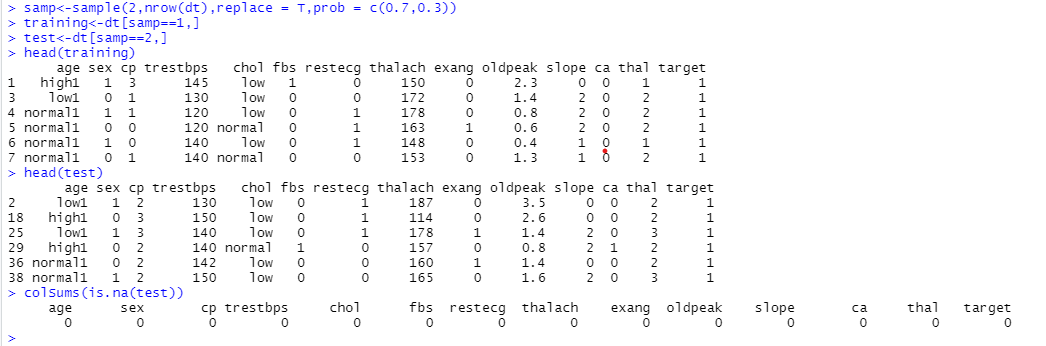
\includegraphics[width=1\textwidth]{task1_1_dataDivide.png}
\end{figure}

\begin{lstlisting}[language=R]
> mod<-glm(target~.,data = training,family = binomial('logit'))
> summary(mod)

Call:
glm(formula = target ~ ., family = binomial("logit"), data = training)

Deviance Residuals: 
    Min       1Q   Median       3Q      Max  
-2.6397  -0.3260   0.1472   0.4614   2.4521  

Coefficients:
              Estimate Std. Error z value Pr(>|z|)   
(Intercept)    1.43597    3.14892   0.456  0.64838   
agenormal1    -1.08551    0.66165  -1.641  0.10088   
agehigh1       0.19073    0.82340   0.232  0.81682   
sex1          -1.27014    0.63533  -1.999  0.04559 * 
cp1            1.07789    0.64981   1.659  0.09716 . 
cp2            1.76202    0.59697   2.952  0.00316 **
cp3            2.33462    0.87380   2.672  0.00754 **
trestbps      -0.02011    0.01359  -1.480  0.13899   
cholnormal    -0.87024    0.56281  -1.546  0.12204   
cholhigh      13.46342 1455.39800   0.009  0.99262   
fbs1           1.40058    0.78331   1.788  0.07377 . 
restecg1       0.75994    0.47349   1.605  0.10850   
restecg2       0.18667    3.24270   0.058  0.95409   
thalach        0.01516    0.01288   1.177  0.23910   
exang1        -1.06170    0.53172  -1.997  0.04585 * 
oldpeak       -0.52696    0.26619  -1.980  0.04774 * 
slope1        -0.74014    1.04764  -0.706  0.47989   
slope2         0.01442    1.13336   0.013  0.98985   
ca            -0.57276    0.23372  -2.451  0.01426 * 
thal1          1.48527    2.16992   0.684  0.49367   
thal2          1.70341    1.83567   0.928  0.35343   
thal3          0.18380    1.87081   0.098  0.92174   
---
Signif. codes:  0 ‘***’ 0.001 ‘**’ 0.01 ‘*’ 0.05 ‘.’ 0.1 ‘ ’ 1

(Dispersion parameter for binomial family taken to be 1)

    Null deviance: 292.99  on 213  degrees of freedom
Residual deviance: 134.65  on 192  degrees of freedom
AIC: 178.65

Number of Fisher Scoring iterations: 14
\end{lstlisting} 
After getting the training model, we need to evaluate the suitability of the model for the scenario by the following metrics
\begin{lstlisting}[language=R]
  predicted<-predict(mod,training,type ="response")
  training$predd<-round(predicted,3)
  View(training)
  ggplot( training, aes( training$predd, color = as.factor(training$target) ) ) + 
    geom_density( ) +
    ggtitle( "Training Set's Predicted Score" )
  training$predw<-ifelse(training$predd>0.46,1,0)
\end{lstlisting}
\begin{figure}[H]
  \centering
  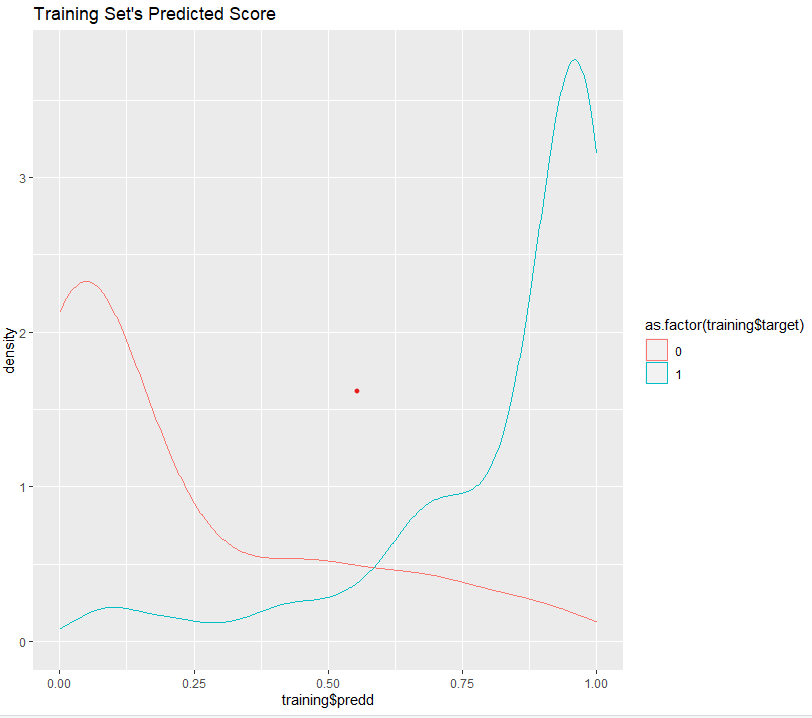
\includegraphics[width=1\textwidth]{task1_1_preScore.png}
\end{figure}

\begin{lstlisting}
> training$predw<-ifelse(training$predd>0.46,1,0)
> confusn<-confusionMatrix(training$target,training$predw,threshold = 0.46)
> confusn
   0   1
0 74  11
1 19 110
> confusn<-as.matrix(confusn)
> AccuracyRate <- sum(diag(confusn))/sum(confusn)
> AccuracyRate
[1] 0.8598131
\end{lstlisting}
Similarly, we need to evaluate this model in the test set
\begin{lstlisting}
> test$prob <- predict(mod,test,type = "response")
> View(test)
> ggplot( test, aes( test$prob, color = as.factor(test$target) ) ) + geom_density( size = 1 ) + ggtitle( "Test Set's Predicted Score" )
> test$predc<-ifelse(test$prob>0.475,1,0)
> confusn<-confusionMatrix(test$target,test$predc,threshold = 0.475)
> confusn
   0  1
0 31  7
1 14 37
> class(confusn)
[1] "data.frame"
> confusn<-as.matrix(confusn)
> AccuracyRate <- sum(diag(confusn))/sum(confusn)
> AccuracyRate
[1] 0.7640449
\end{lstlisting}
\begin{figure}[H]
  \centering
  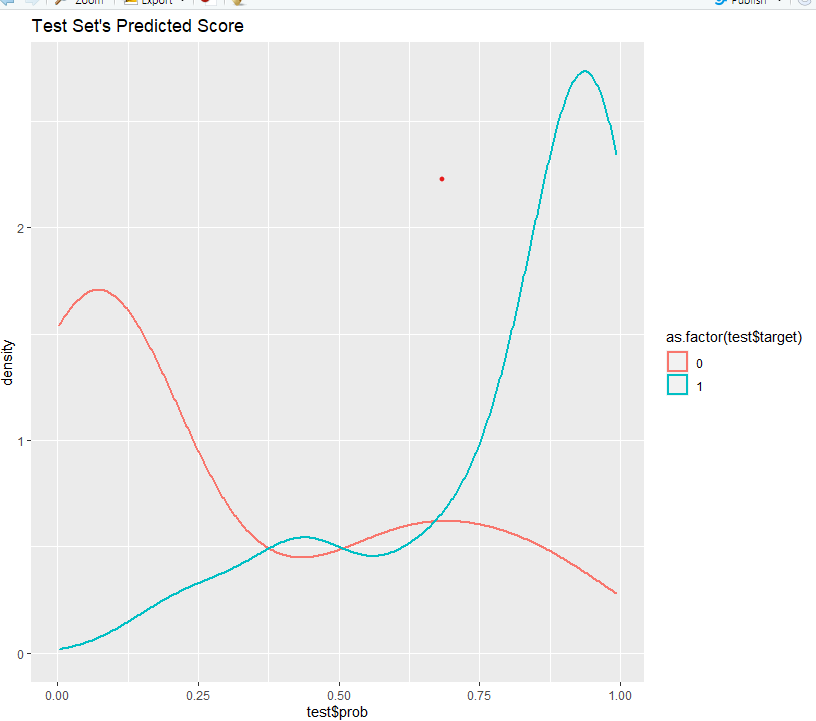
\includegraphics[width=1\textwidth]{task1_1_testScore.png}
\end{figure}
The evaluation summary of logistic regression can be seen below
\begin{lstlisting}
  > Confusion
         Actual
Predicted  0  1
        0 31  7
        1 14 37
> AccuracyRate
[1] 0.7640449
> plot(rocCurve)
> rocCurve$sensitivities
[1] 1.0000000 0.6888889 0.0000000
> rocCurve$specificities
[1] 0.0000000 0.8409091 1.0000000
> rocCurve$au
Area under the curve: 0.7649
\end{lstlisting}

\subsection{method2}
\subsection{method3}
\subsection{discuss}
\section{Task3}
\subsection{Data mining and cleaning}
This data comes from Twitter sentiment analysis in kaggle, From a data set of nearly one million, 13,700 comments about Alan bryd were selected. Among these data, 9,700 positive sentiment data. 4000 negative emotion data. In order to balance the data set, 4000 positive sentiment data and 4000 negative sentiment data were extracted.
 \begin{figure}[H]
\centering
  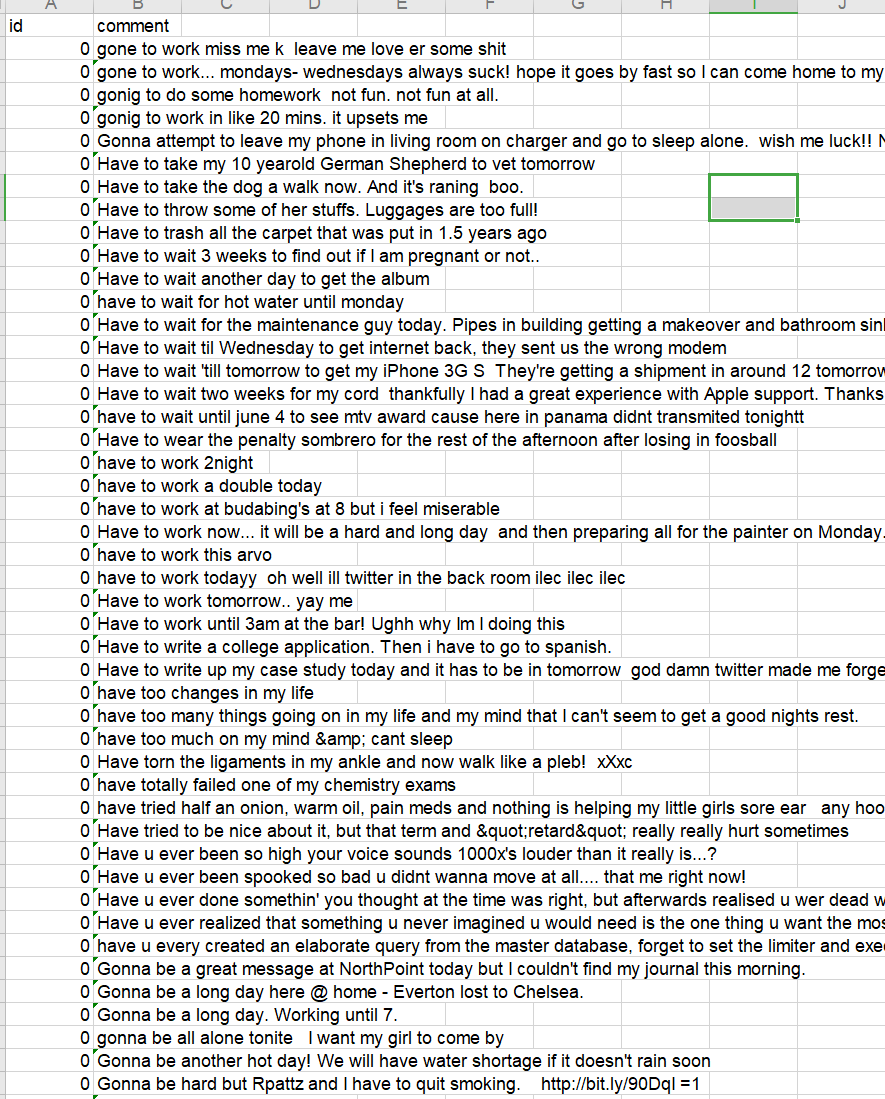
\includegraphics[width=.8\textwidth]{3-1.png} %1.png是图片文件的相对路径

\end{figure}
There are most characters in the comments, such as emoji, @ other users and some garbled characters are inconsistent in capitalization
 \begin{figure}[H]
\centering
  
\includegraphics[width=.8\textwidth]{3-2.png} %1.png是图片文件的相对路径
  \end{figure}
So a series of data cleaning operations are used to clean the data.
 \begin{figure}[H]
\centering
  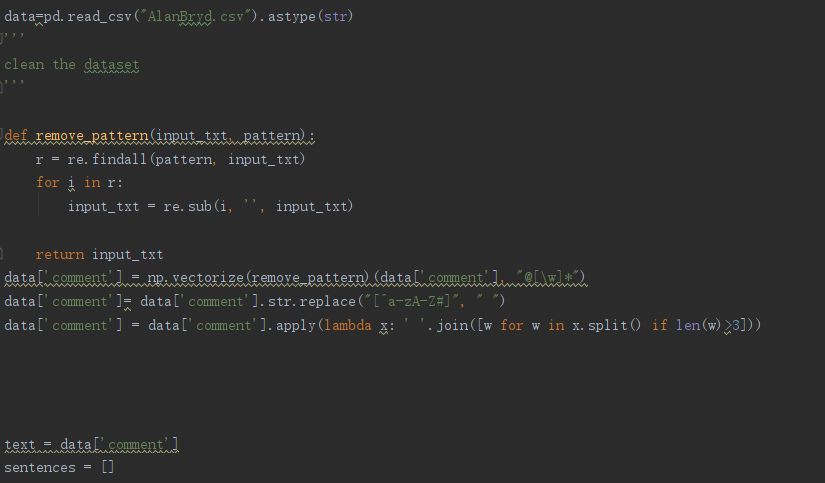
\includegraphics[width=.8\textwidth]{3-3.png} %1.png是图片文件的相对路径
  \end{figure}
\subsection{Use word2vec to build word vectors}
 \begin{figure}[H]
\centering
  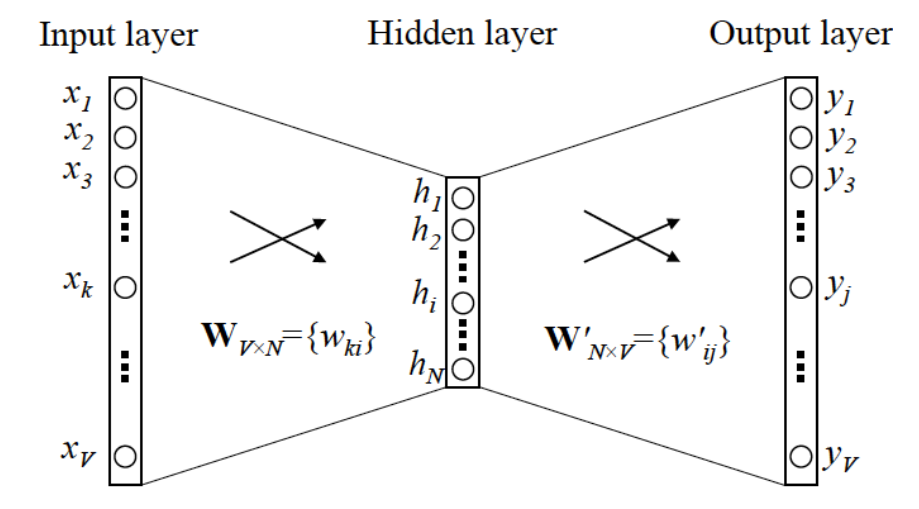
\includegraphics[width=.8\textwidth]{3-4.png} %1.png是图片文件的相对路径
  \end{figure}
Use word2vec's word vector for word embedding as input to the model
 \begin{figure}[H]
\centering
  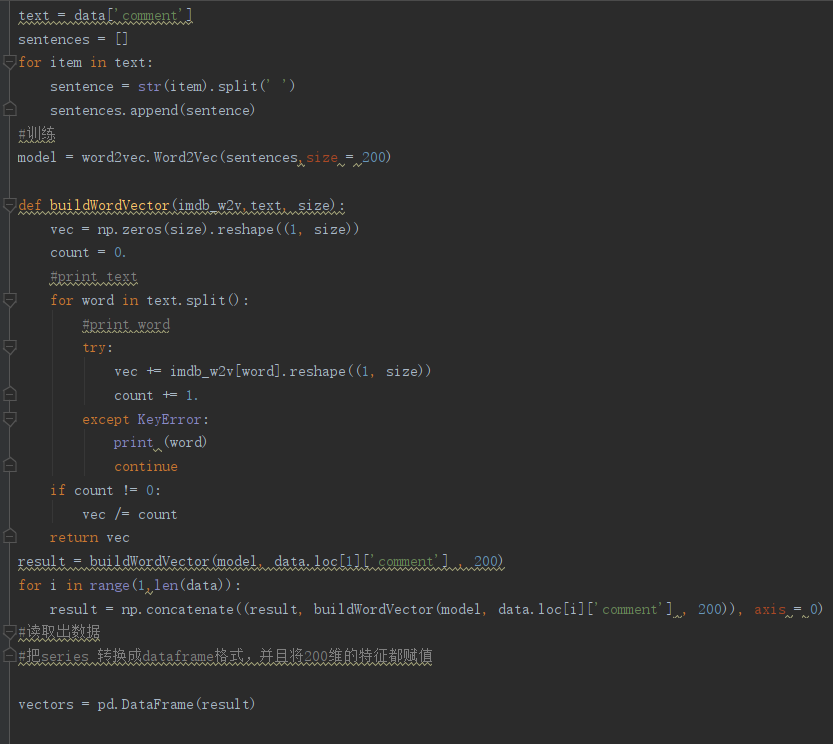
\includegraphics[width=.8\textwidth]{3-5.png} %1.png是图片文件的相对路径
  \end{figure}
\subsection{model using and result}
\subsubsection{GBDT}
theory of GBDT
 \begin{figure}[H]
\centering
  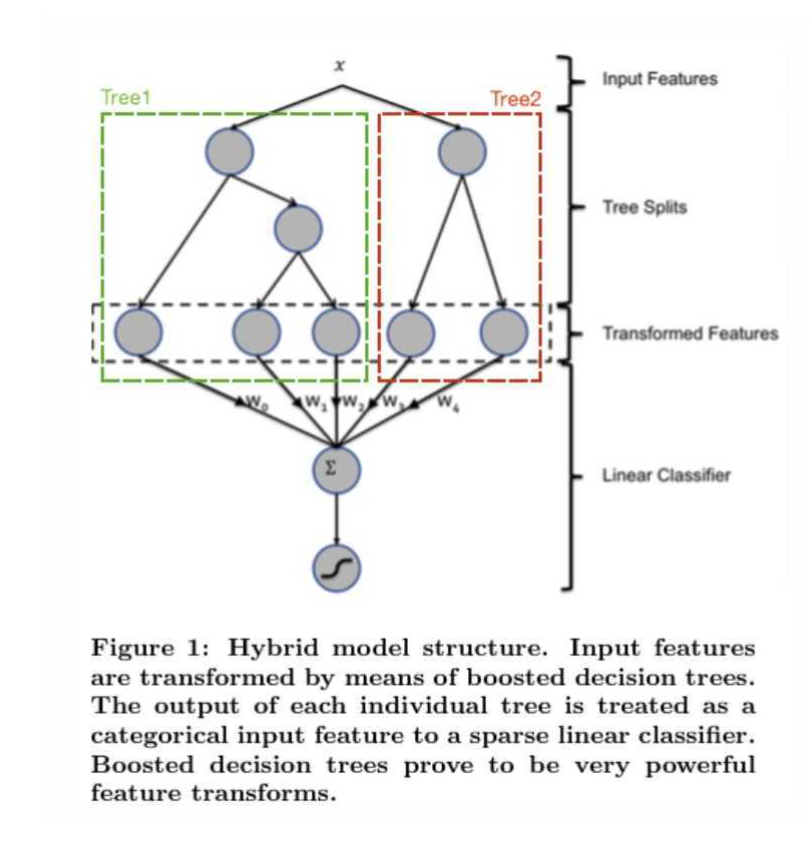
\includegraphics[width=.8\textwidth]{3-6.png} %1.png是图片文件的相对路径
  \end{figure}
Parameters of gbdt:\\
    $n_estimators=1000,$
    $subsample=0.8,$
    $loss='deviance',$
    $max_features='sqrt',$

  \subsubsection{SVM}
 theory of SVM
  \begin{figure}[H]
\centering
  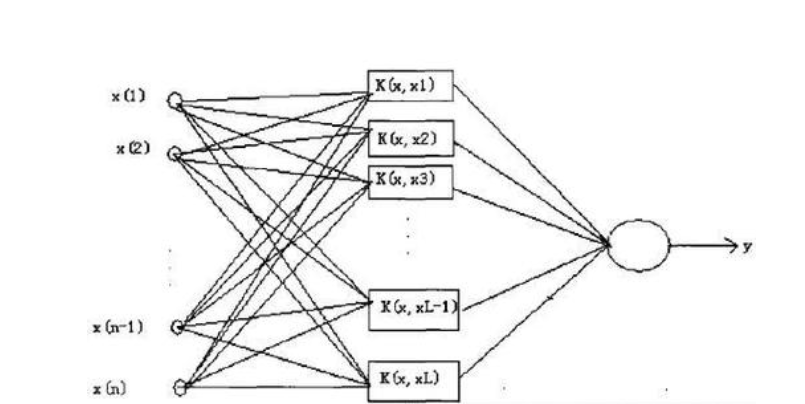
\includegraphics[width=.8\textwidth]{3-7.png} %1.png是图片文件的相对路径
  \end{figure}
Parameters of SVM:
$
kernel=‘rbf’
degree=3
$
\subsubsection{RandomForest}
 theory of RF
   \begin{figure}[H]
\centering
  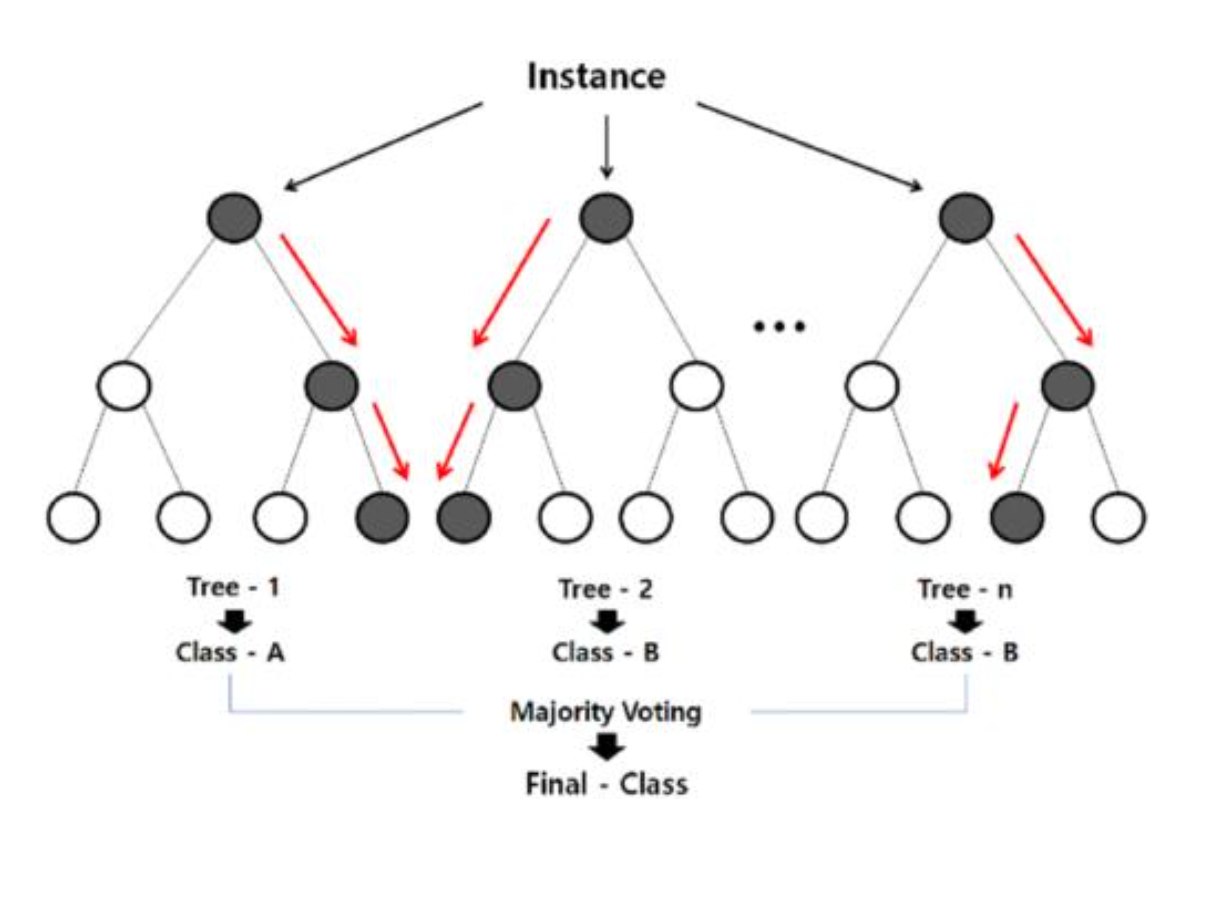
\includegraphics[width=.8\textwidth]{3-8.png} %1.png是图片文件的相对路径
  \end{figure}
Parameters of RF:$
    oob_score=True,
    n_estimators=400,
    max_features='sqrt',
    $
\subsubsection{ExtraTrees}
theory of ET
   \begin{figure}[H]
\centering
  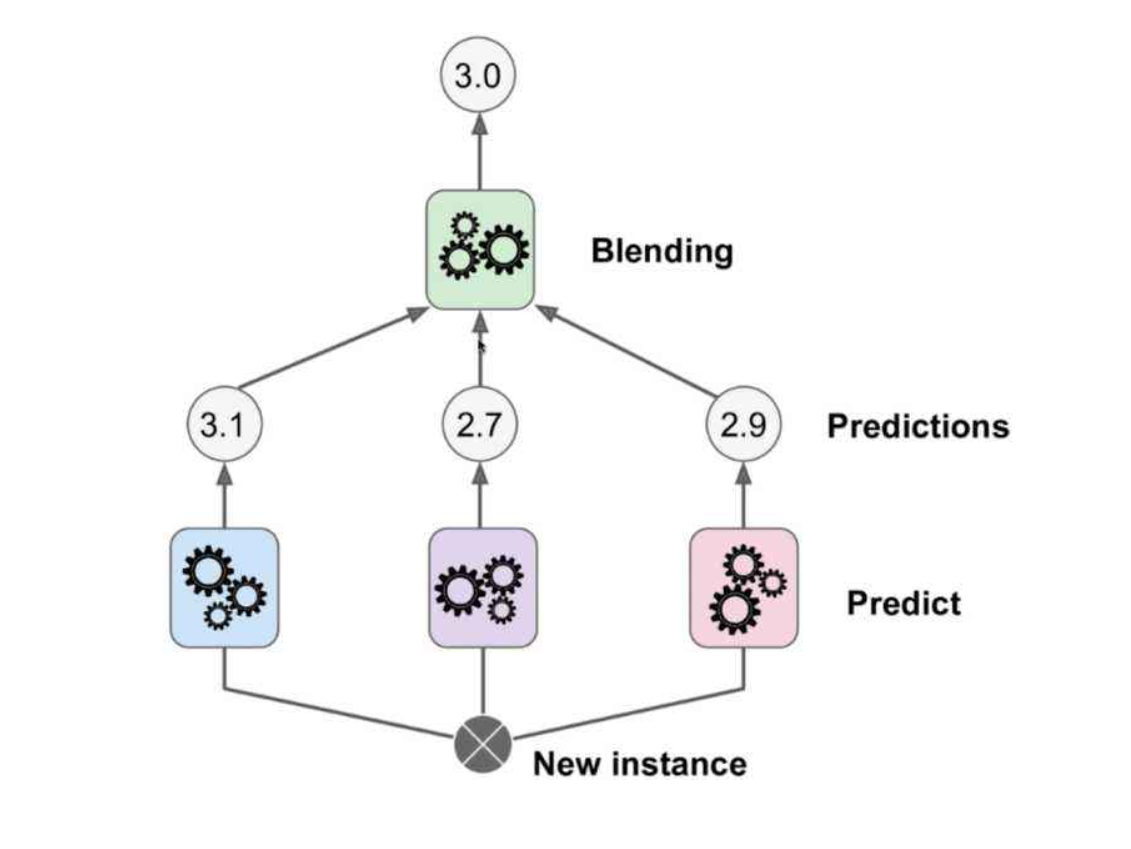
\includegraphics[width=.8\textwidth]{3-9.png} %1.png是图片文件的相对路径
  \end{figure}
 Parameter of ET:
 $
 criterion=gini,
 max features=log,
 max depth=50
 $
 \subsubsection{Result}
    \begin{figure}[H]
\centering
  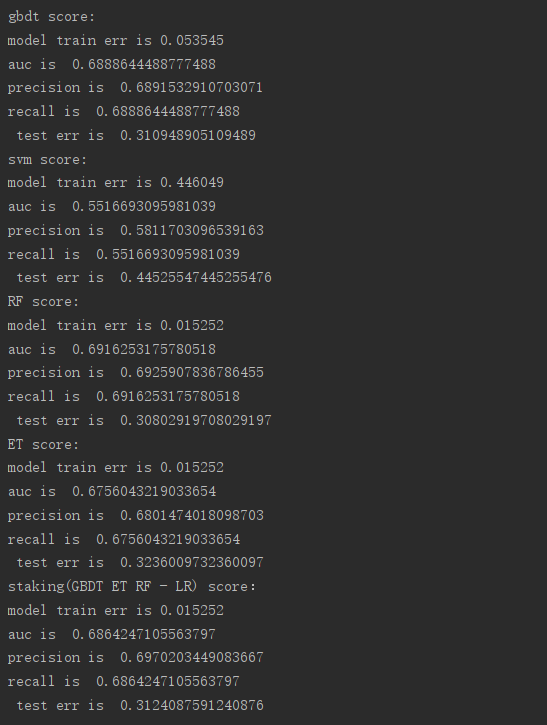
\includegraphics[width=.8\textwidth]{3-10.png} %1.png是图片文件的相对路径
  \end{figure}
According to the picture above,The expressive power of gbdt is better than other models in all aspects, and the mathematical model in machine learning can fit the features well when the data set is not large. Compared with other tree models, GBDT has a stronger ability to fit data by calculating residuals.
The auc figure of GBDT is :
    \begin{figure}[H]
\centering
  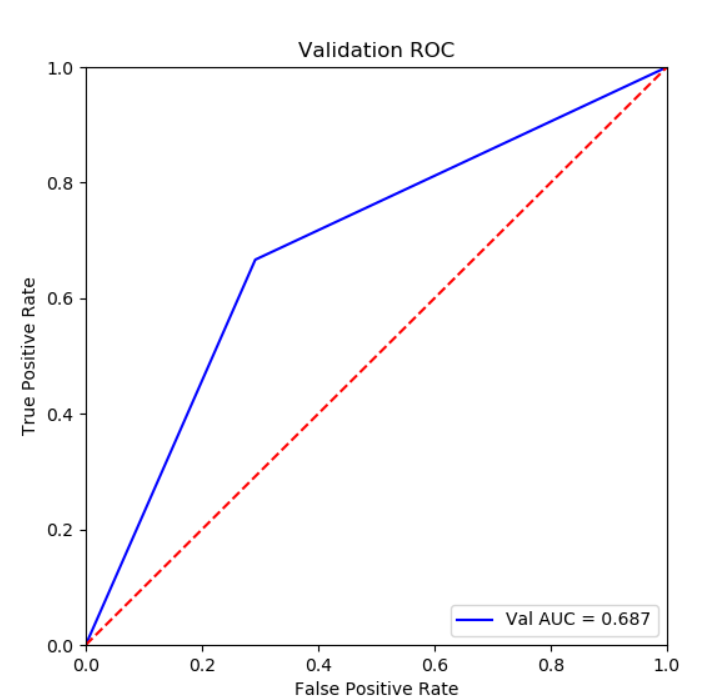
\includegraphics[width=.8\textwidth]{3-11.png} %1.png是图片文件的相对路径
  \end{figure}
\end{document}
